\documentclass[11pt]{beamer}\usepackage[]{graphicx}\usepackage[]{color}
%% maxwidth is the original width if it is less than linewidth
%% otherwise use linewidth (to make sure the graphics do not exceed the margin)
\makeatletter
\def\maxwidth{ %
  \ifdim\Gin@nat@width>\linewidth
    \linewidth
  \else
    \Gin@nat@width
  \fi
}
\makeatother

\definecolor{fgcolor}{rgb}{0.345, 0.345, 0.345}
\newcommand{\hlnum}[1]{\textcolor[rgb]{0.686,0.059,0.569}{#1}}%
\newcommand{\hlstr}[1]{\textcolor[rgb]{0.192,0.494,0.8}{#1}}%
\newcommand{\hlcom}[1]{\textcolor[rgb]{0.678,0.584,0.686}{\textit{#1}}}%
\newcommand{\hlopt}[1]{\textcolor[rgb]{0,0,0}{#1}}%
\newcommand{\hlstd}[1]{\textcolor[rgb]{0.345,0.345,0.345}{#1}}%
\newcommand{\hlkwa}[1]{\textcolor[rgb]{0.161,0.373,0.58}{\textbf{#1}}}%
\newcommand{\hlkwb}[1]{\textcolor[rgb]{0.69,0.353,0.396}{#1}}%
\newcommand{\hlkwc}[1]{\textcolor[rgb]{0.333,0.667,0.333}{#1}}%
\newcommand{\hlkwd}[1]{\textcolor[rgb]{0.737,0.353,0.396}{\textbf{#1}}}%

\usepackage{framed}
\makeatletter
\newenvironment{kframe}{%
 \def\at@end@of@kframe{}%
 \ifinner\ifhmode%
  \def\at@end@of@kframe{\end{minipage}}%
  \begin{minipage}{\columnwidth}%
 \fi\fi%
 \def\FrameCommand##1{\hskip\@totalleftmargin \hskip-\fboxsep
 \colorbox{shadecolor}{##1}\hskip-\fboxsep
     % There is no \\@totalrightmargin, so:
     \hskip-\linewidth \hskip-\@totalleftmargin \hskip\columnwidth}%
 \MakeFramed {\advance\hsize-\width
   \@totalleftmargin\z@ \linewidth\hsize
   \@setminipage}}%
 {\par\unskip\endMakeFramed%
 \at@end@of@kframe}
\makeatother

\definecolor{shadecolor}{rgb}{.97, .97, .97}
\definecolor{messagecolor}{rgb}{0, 0, 0}
\definecolor{warningcolor}{rgb}{1, 0, 1}
\definecolor{errorcolor}{rgb}{1, 0, 0}
\newenvironment{knitrout}{}{} % an empty environment to be redefined in TeX

\usepackage{alltt}
\usetheme{Warsaw}
\usepackage[utf8]{inputenc}
\usepackage{amsmath}
\usepackage{amsfonts}
\usepackage{amssymb}
\usepackage{array}
\usepackage{graphicx}
\author{John Muschelli}
\usepackage{hyperref}
\setbeamertemplate{navigation symbols}{}%remove navigation symbols

\title{Displaying Image Information}
%\setbeamercovered{transparent} 
%\setbeamertemplate{navigation symbols}{} 
%\logo{} 
\institute{Johns Hopkins Bloomberg School of Public Health} 
%\date{} 
%\subject{} 
\setlength{\topsep}{0pt}
\setlength{\parskip}{0pt}
\setlength{\partopsep}{1pt}
\setbeamertemplate{footline}[frame number]

\newcommand {\framedgraphic}[2] {
    \begin{frame}{#1}
        \begin{center}
            \includegraphics[width=\textwidth,height=0.8\textheight,keepaspectratio]{#2}
        \end{center}
    \end{frame}
}
\IfFileExists{upquote.sty}{\usepackage{upquote}}{}
\begin{document}

\begin{frame}
\titlepage
\end{frame}

%\begin{frame}
%\tableofcontents
%\end{frame}



\begin{frame}[fragile]{Reading In Data}
The \verb|readNIfTI| command (\verb|oro.nifti| package) can read in NIfTI file (compressed or not) into a \verb|nifti| object.  We will read in the NIfTI (T1-weighted) image from the previous session:

\begin{knitrout}
\definecolor{shadecolor}{rgb}{0.969, 0.969, 0.969}\color{fgcolor}\begin{kframe}
\begin{alltt}
\hlkwd{library}\hlstd{(oro.nifti)}
\hlkwd{print}\hlstd{(\{nii} \hlkwb{=} \hlkwd{readNIfTI}\hlstd{(}\hlkwc{fname} \hlstd{=} \hlstr{"Output_3D_File"}\hlstd{)\})}
\end{alltt}
\begin{verbatim}
NIfTI-1 format
  Type            : nifti
  Data Type       : 4 (INT16)
  Bits per Pixel  : 16
  Slice Code      : 0 (Unknown)
  Intent Code     : 0 (None)
  Qform Code      : 2 (Aligned_Anat)
  Sform Code      : 2 (Aligned_Anat)
  Dimension       : 512 x 512 x 22
  Pixel Dimension : 0.47 x 0.47 x 5
  Voxel Units     : mm
  Time Units      : sec
\end{verbatim}
\end{kframe}
\end{knitrout}
\end{frame}

\begin{frame}[fragile]{Visualizing a Slice}
The \verb|nifti| object is a 3D \verb|array| (see \verb|?array|) with header information.  We can use the \verb|image| function (\verb|graphics| package) to visualize a slice (slice 20 in the z-direction/axial):

\begin{center}
\begin{knitrout}
\definecolor{shadecolor}{rgb}{0.969, 0.969, 0.969}\color{fgcolor}\begin{kframe}
\begin{alltt}
\hlkwd{image}\hlstd{(nii[,,}\hlnum{20}\hlstd{])}
\end{alltt}
\end{kframe}
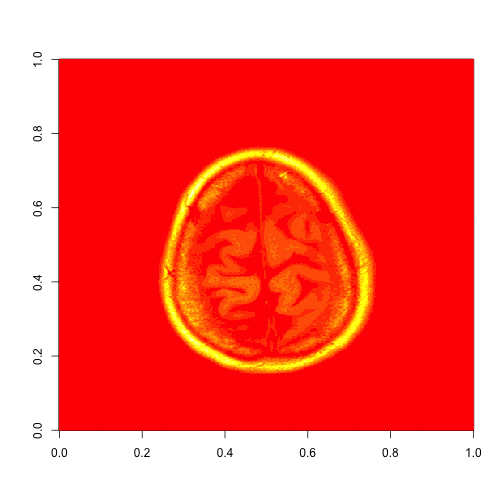
\includegraphics[width=\textwidth,height=0.5\textheight,keepaspectratio]{figure/image1-1} 

\end{knitrout}
\end{center}

\end{frame}


\begin{frame}[fragile]{Visualizing a Slice}
\verb|graphics::image| uses \verb|heat.colors(12)| for coloring, which is not useful for this task.  We can either set the colors manually, or use the \verb|oro.nifti::image| function.  The function is still \verb|image|, but we don't pass in a  slice, but the \verb|nifti| object and specify the slice \verb|z=20|:

\begin{center}
\begin{knitrout}
\definecolor{shadecolor}{rgb}{0.969, 0.969, 0.969}\color{fgcolor}\begin{kframe}
\begin{alltt}
\hlkwd{image}\hlstd{(nii,} \hlkwc{z} \hlstd{=} \hlnum{20}\hlstd{,} \hlkwc{plot.type}\hlstd{=}\hlstr{'single'}\hlstd{)}
\end{alltt}
\end{kframe}
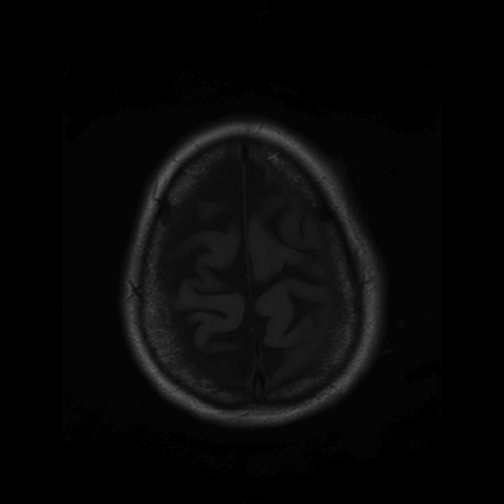
\includegraphics[width=\textwidth,height=0.5\textheight,keepaspectratio]{figure/image_nifti-1} 

\end{knitrout}
\end{center}

% \framedgraphic{figure/image.nifti-1.png}

\end{frame}


\begin{frame}[fragile]{Visualizing a Slice}
If \verb|plot.type| is not \verb|'single'|, \verb|image.nifti| defaults to plotting ALL slices with data, even if \verb|z| is specified (also called a ``lightbox''):

\begin{center}
\begin{knitrout}
\definecolor{shadecolor}{rgb}{0.969, 0.969, 0.969}\color{fgcolor}\begin{kframe}
\begin{alltt}
\hlkwd{image}\hlstd{(nii,} \hlkwc{z} \hlstd{=} \hlnum{20}\hlstd{)}
\end{alltt}
\end{kframe}
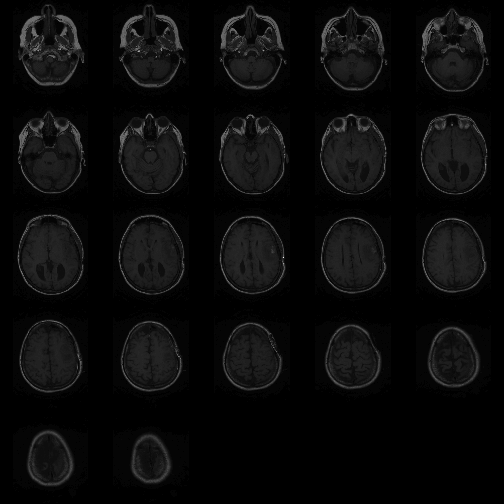
\includegraphics[width=\textwidth,height=0.5\textheight,keepaspectratio]{figure/image_mult-1} 

\end{knitrout}
\end{center}

\end{frame}

\begin{frame}[fragile]{Visualizing all 3 planes}
To show all 3 planes (axial, sagittal, and coronal) of an image, we can use the \verb|orthographic| function:

\begin{center}
\begin{knitrout}
\definecolor{shadecolor}{rgb}{0.969, 0.969, 0.969}\color{fgcolor}\begin{kframe}
\begin{alltt}
\hlkwd{orthographic}\hlstd{(nii)}
\end{alltt}
\end{kframe}
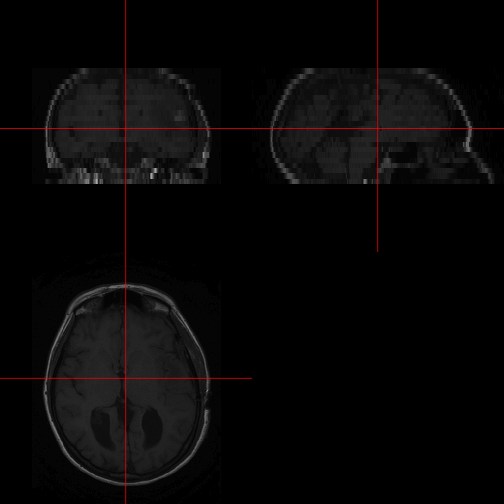
\includegraphics[width=\textwidth,height=0.5\textheight,keepaspectratio]{figure/image_ortho-1} 

\end{knitrout}
\end{center}

\end{frame}


\begin{frame}[fragile]{Histograms}
What about the {\bf data}?  We can do normal operations, such as histograms of the image intensities and intensities over $20$:

\begin{center}
\begin{knitrout}
\definecolor{shadecolor}{rgb}{0.969, 0.969, 0.969}\color{fgcolor}\begin{kframe}
\begin{alltt}
\hlkwd{par}\hlstd{(}\hlkwc{mfrow}\hlstd{=}\hlkwd{c}\hlstd{(}\hlnum{1}\hlstd{,}\hlnum{2}\hlstd{));}
\hlkwd{hist}\hlstd{(nii,} \hlkwc{breaks} \hlstd{=} \hlnum{2000}\hlstd{);} \hlkwd{hist}\hlstd{(nii[nii} \hlopt{>} \hlnum{20}\hlstd{],} \hlkwc{breaks} \hlstd{=} \hlnum{2000}\hlstd{)}
\end{alltt}
\end{kframe}
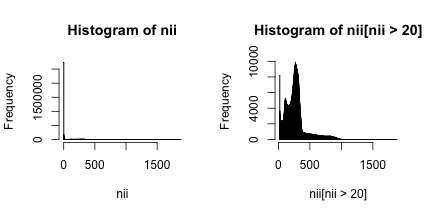
\includegraphics[width=\textwidth,height=0.5\textheight,keepaspectratio]{figure/image_hist-1} 

\end{knitrout}
\end{center}

\end{frame}

\begin{frame}[fragile]{Image Overlays}
We can do overlays as well, where we have one image and color it by a second.  For example, we plot slice $10$ and highlight values between $300$ and $400$ (next slide we discuss the code):

\begin{center}
\begin{knitrout}
\definecolor{shadecolor}{rgb}{0.969, 0.969, 0.969}\color{fgcolor}\begin{kframe}
\begin{alltt}
\hlkwd{library}\hlstd{(fslr)} \hlcom{# need niftiarr}
\hlstd{mask} \hlkwb{=} \hlstd{fslr}\hlopt{::}\hlkwd{niftiarr}\hlstd{(nii, nii} \hlopt{>} \hlnum{300} \hlopt{&} \hlstd{nii} \hlopt{<} \hlnum{400}\hlstd{)}
\hlstd{mask[mask} \hlopt{==} \hlnum{0}\hlstd{]} \hlkwb{=} \hlnum{NA}
\hlkwd{overlay}\hlstd{(nii, mask,} \hlkwc{col.y}\hlstd{=} \hlkwd{c}\hlstd{(}\hlstr{"red"}\hlstd{),}
        \hlkwc{plot.type}\hlstd{=}\hlstr{"single"}\hlstd{,} \hlkwc{z} \hlstd{=} \hlnum{10}\hlstd{)}
\end{alltt}
\end{kframe}
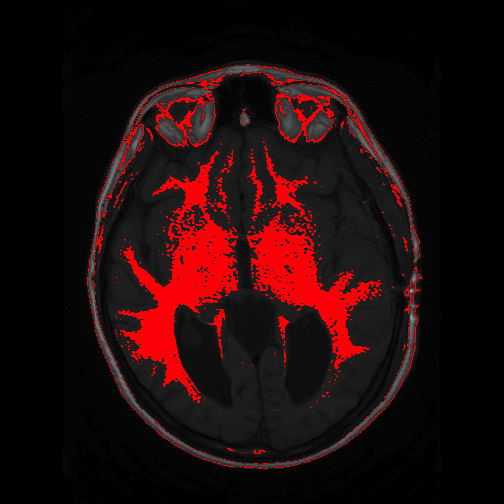
\includegraphics[width=\textwidth,height=0.5\textheight,keepaspectratio]{figure/image_overlay-1} 

\end{knitrout}
\end{center}

\end{frame}


\begin{frame}[fragile]{Image Overlays: Explained}
We load the \verb|fslr| package, which has helper functions for \verb|nifti| objects.  The \verb|nii > 300 & nii < 400| operation returns an \verb|array|, not \verb|nifti| object.  The \verb|niftiarr| command takes in a \verb|nifti| object and array and returns a \verb|nifti| object with the array in the data slot.  We then set any $0$ in mask to \verb|NA| so the \verb|overlay| (\verb|oro.nifti package|) will not mask out data.
\begin{center}
\begin{knitrout}
\definecolor{shadecolor}{rgb}{0.969, 0.969, 0.969}\color{fgcolor}\begin{kframe}
\begin{alltt}
\hlkwd{library}\hlstd{(fslr)} \hlcom{# need niftiarr}
\hlstd{mask} \hlkwb{=} \hlstd{fslr}\hlopt{::}\hlkwd{niftiarr}\hlstd{(nii, nii} \hlopt{>} \hlnum{300} \hlopt{&} \hlstd{nii} \hlopt{<} \hlnum{400}\hlstd{)}
\hlstd{mask[mask} \hlopt{==} \hlnum{0}\hlstd{]} \hlkwb{=} \hlnum{NA}
\hlkwd{overlay}\hlstd{(nii, mask,} \hlkwc{col.y}\hlstd{=} \hlkwd{c}\hlstd{(}\hlstr{"red"}\hlstd{),}
        \hlkwc{plot.type}\hlstd{=}\hlstr{"single"}\hlstd{,} \hlkwc{z} \hlstd{=} \hlnum{10}\hlstd{)}
\end{alltt}
\end{kframe}
\end{knitrout}
\end{center}

\end{frame}

\begin{frame}[fragile]{Image Overlays: 3 Planes}
We can perform the same operation of overlaying, but in all 3 planes:
\begin{center}
\begin{knitrout}
\definecolor{shadecolor}{rgb}{0.969, 0.969, 0.969}\color{fgcolor}\begin{kframe}
\begin{alltt}
\hlkwd{orthographic}\hlstd{(nii, mask,} \hlkwc{col.y}\hlstd{=} \hlkwd{c}\hlstd{(}\hlstr{"red"}\hlstd{),}
             \hlkwc{text} \hlstd{=}\hlstr{"Image overlaid with mask"}\hlstd{)}
\end{alltt}
\end{kframe}
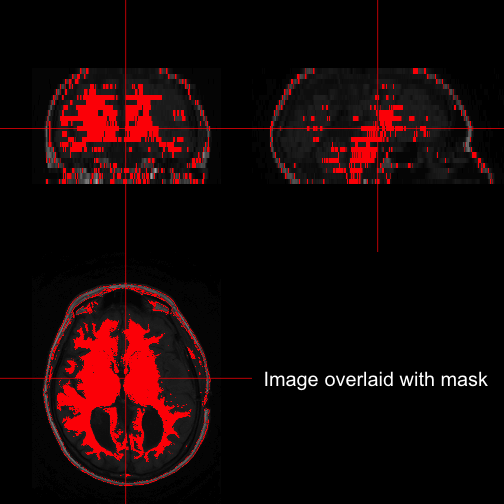
\includegraphics[width=\textwidth,height=0.5\textheight,keepaspectratio]{figure/image_ortho_overlay-1} 

\end{knitrout}
\end{center}

\end{frame}


\begin{frame}[fragile]{Functions discussed here}
\begin{itemize}
\item \verb|readNIfTI|: read in data
\item \verb|graphics::image|: display matrix data
\item \verb|oro.nifti::image|: display \verb|nifti| data
\item \verb|oro.nifti::orthographic|: display 3-planes of an image
\item \verb|oro.nifti::overlay|: display overlay of 2 images (NA are not plotting in \verb|y| image)
\item \verb|fslr::niftiarr(x,y|: Copy \verb|nifti| header from object \verb|x| and put in new \verb|array| \verb|y| into data part
\end{itemize}

\end{frame}





\end{document}
